\section{Matrices Ralas}

Una forma posible de almancenar los tractogramas es convertir cada uno a un 
vector fila y almacenarlos todos juntos en una misma matriz. En nuestro caso,
hacer esto con los tractogramas del \'Area de Broca gener\'o una matriz de
dimensiones $762\times3587328$. Asumiendo que cada valor se representa usando 
$8$ Bytes en memoria, esta matriz ocupa un total de aproximadamente $20$ Gigabytes.
Sin embargo, solo un $1\%$ de los datos almancenados resultaron ser no nulos. 
Casi todo el espacio utilizado es desperdiciado.\\

Es posible mejorar esto eliminando de la matriz las columnas que poseen solo
elementos nulos. La Figura \ref{fig:densa} muestra la matriz que resulta de aplicar
este procedimiento a los tractogramas del \'Area de Broca. Si bien la nueva
matriz posee dimensiones $762\times121045$, a\'un solo el $27\%$ de los valores 
almacenados son no nulos. Manteniendo la representaci\'on de $8$ Bytes es posible
reducir el espacio necesario de $20\%$ Gigabites a aproximadamente $700$ Megabytes.\\

\begin{figure}[h!]
   \centering
    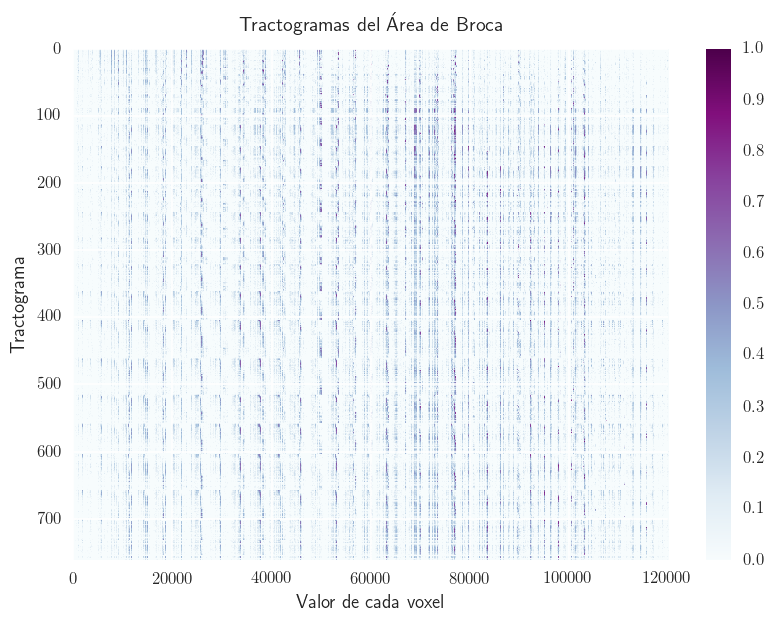
\includegraphics[width=\textwidth]{img/densa_broca.png}
    \caption{Semillas en el hemisferio izquierdo. }
    \label{fig:densa}
\end{figure}

El problema de este \'ultimo m\'etodo es que a\'un desperdicia mucho espacio. En
el caso de utilizar todas los tractogramas de un hemisferio, la matriz pasa a ser
de dimensiones $21657\times3587328$ con un $1\%$ de valores no nulos. Para almacenar
dicha matriz es necesario utilizar $587$ Gigabytes. Por esto es necesario
utilizar estructuras mas eficiente, como un \textit{Dictionary of Keys}, o
una matriz \textit{Compressed Sparse Row} (CSR). \\

%eliminando columnas inutiles nos queda 21657x145574, son 23.5 Gn

El \textit{Dictionary of Keys} (DOK) representa una matriz mediante un diccionario.
Almacena los valores de la matriz indexandolos con las coordenadas de su matriz.
Todas aquellas coordenadas que no poseen un valor asociado se asumen nulas. Esta 
estructura se suele utilizar para crear las matrices ralas. Luego, para realizar
operaciones con las mismas, resulta mas eficiente transformarlas a CSR. \\

\textit{Compressed Sparse Row} es otra manera de representar matrices
ralas. En este caso se utilizan tres vectores comunmente denominados $A$, $IA$ y
$JA$. $A$ posee todos los valores no nulos; los valores de $A$ entre los indices
$IA_i$ e $IA_{i+1}-1$ son los valores no nulos de la fila $i$. Finalmente, $JA_i$
posee el numero de columna al cual pertenece $A_i$. Por ejemplo, para la siguiente
matriz $M$:

$$
    M =
    \begin{pmatrix}
             0 & 0 & 0 & 0 \\
             5 & 8 & 3 & 0 \\
             0 & 6 & 0 & 0    
    \end{pmatrix}
$$    

$$ A  = \begin{pmatrix} 5 & 8 & 3 & 6     \end{pmatrix} $$
$$ IA = \begin{pmatrix} 0 & 0 & 2 & 3 & 4 \end{pmatrix} $$
$$ JA = \begin{pmatrix} 0 & 1 & 2 & 1     \end{pmatrix} $$

CSR permite realizar sumas, multiplicaciones y operaciones con sus filas de manera
eficiente. 

BUSCAR REFERENCIAS PARA TODO ESTO.
